%% FullCourse_10Lecs -- Lecture 1, Topic 1.3: How This Course Works
%% New deck for the re-pitched "Introduction" lecture.
%% Reuses roadmap / two-arcs / 10-lecture-map / economists-bring frames from the
%% old Lec02_T2_Cognitive_Capital_Roadmap.tex; new tooling + capstone content from
%% Docs/Capstone_Projects_2026.md and Labs/README.md.

%% Shared preamble for the FullCourse_10Lecs topic decks.
%%
%% Each topic .tex \input's this file, then defines its own \title, \date
%% override (if any), \graphicspath, and \begin{document}.
%%
%% Reconstructed verbatim from the inlined copy preserved in
%% Lec10_Case_Studies/Lec10_T8_Case6_DeepRamsey.tex (lines 23-190), which is
%% explicitly annotated there as "from ../shared_preamble.tex, copied verbatim".
%% Base preamble matches MiniCourse_8hr/Slides/shared_preamble.tex; this version
%% additionally provides \sectiondivider, the conceptbox/cautionbox/examplebox/
%% takeawaybox tcolorboxes, and \compacttables used across the split decks.

\documentclass[10pt,english,aspectratio=169]{beamer}

\usepackage{ae,aecompl}
\usepackage[T1]{fontenc}
\usepackage{textcomp}
\usepackage[utf8]{inputenc}
\usepackage{babel}
\usepackage{datetime2}

\setcounter{secnumdepth}{3}
\setcounter{tocdepth}{3}

\usepackage{amsmath, amssymb, amsthm, graphicx}
\usepackage{booktabs, multirow}
\usepackage{tikz}
\usepackage{pgfplots}
\pgfplotsset{compat=1.16}
\usepackage[most]{tcolorbox}
\tcbuselibrary{skins, breakable, theorems}
\usepackage{listings}
\usepackage{xcolor}

\lstset{
  basicstyle=\ttfamily\small,
  keywordstyle=\color{blue!80!black}\bfseries,
  commentstyle=\color{green!50!black}\itshape,
  stringstyle=\color{orange!80!black},
  backgroundcolor=\color{gray!8},
  frame=single,
  rulecolor=\color{gray!40},
  breaklines=true,
  showstringspaces=false,
  numbers=none,
}

\lstdefinestyle{pythonstyle}{
    language=Python,
    basicstyle=\ttfamily\footnotesize,
    keywordstyle=\color{blue!80!black}\bfseries,
    commentstyle=\color{green!50!black}\itshape,
    stringstyle=\color{orange!80!black},
    frame=single,
    breaklines=true,
    showstringspaces=false,
    numbers=left,
    numbersep=5pt,
    numberstyle=\tiny\color{gray},
    backgroundcolor=\color{gray!8},
    rulecolor=\color{gray!40}
}

\ifx\hypersetup\undefined
  \AtBeginDocument{%
    \hypersetup{bookmarks=false,breaklinks=true,pdfborder={0 0 0},colorlinks=true,
      linkcolor=DarkText,urlcolor=RedTitle}%
  }
\else
  \hypersetup{bookmarks=false,breaklinks=true,pdfborder={0 0 0},colorlinks=true,
    linkcolor=DarkText,urlcolor=RedTitle}%
\fi

\makeatletter
\newcommand\makebeamertitle{%
  \begin{frame}[plain]
    \vspace*{1.0cm}
    \centering
    {\usebeamerfont{title}\usebeamercolor[fg]{title}\inserttitle\par}
    \vspace{1.0cm}
    {\usebeamerfont{author}\usebeamercolor[fg]{author}\insertauthor\par}
    \vspace{0.2cm}
    {\usebeamerfont{date}\usebeamercolor[fg]{date}\insertdate\par}
  \end{frame}}%
\AtBeginDocument{%
  \let\origtableofcontents=\tableofcontents
  \def\tableofcontents{\@ifnextchar[{\origtableofcontents}{\gobbletableofcontents}}
  \def\gobbletableofcontents#1{\origtableofcontents}%
}

\usetheme{metropolis}
\usefonttheme{professionalfonts}

\definecolor{LightGray}{RGB}{230,230,230}
\definecolor{RedTitle}{RGB}{0,0,200}
\definecolor{VeryLightGray}{RGB}{245,245,245}
\definecolor{DarkText}{RGB}{0,0,0}

\setbeamercolor{background canvas}{bg=white}
\setbeamercolor{title}{fg=RedTitle}
\setbeamercolor{author}{fg=DarkText}
\setbeamercolor{date}{fg=DarkText}
\setbeamercolor{frametitle}{bg=VeryLightGray,fg=DarkText}
\setbeamercolor{normal text}{fg=DarkText}
\setbeamerfont{title}{size=\large}

\setbeamersize{text margin left=5mm, text margin right=5mm}
\addtobeamertemplate{frametitle}{}{\vspace{-0.5em}}
\newcommand{\reducevspace}{\vspace{-0.5cm}}

% Shared section divider and box styles for split topic decks.
\newcommand{\sectiondivider}[2]{%
\begin{frame}[plain,noframenumbering]
\begin{center}
\vfill
{\Large\textbf{#1}\par}
\vspace{0.35cm}
{\normalsize #2\par}
\vfill
\end{center}
\end{frame}
}

\newtcolorbox{conceptbox}[1][]{
  colback=blue!3,
  colframe=RedTitle!55,
  boxrule=0.35mm,
  arc=1mm,
  left=2mm,
  right=2mm,
  top=1mm,
  bottom=1mm,
  #1
}
\newtcolorbox{cautionbox}[1][]{
  colback=red!3,
  colframe=red!50!black,
  boxrule=0.35mm,
  arc=1mm,
  left=2mm,
  right=2mm,
  top=1mm,
  bottom=1mm,
  #1
}
\newtcolorbox{examplebox}[1][]{
  colback=green!3,
  colframe=green!45!black,
  boxrule=0.35mm,
  arc=1mm,
  left=2mm,
  right=2mm,
  top=1mm,
  bottom=1mm,
  #1
}
\newtcolorbox{takeawaybox}[1][]{
  colback=VeryLightGray,
  colframe=RedTitle!55,
  boxrule=0.35mm,
  arc=1mm,
  left=2mm,
  right=2mm,
  top=1mm,
  bottom=1mm,
  #1
}
\newcommand{\compacttables}{\renewcommand{\arraystretch}{1.15}}

\setbeamertemplate{navigation symbols}{}
\setbeamertemplate{footline}{%
  \hfill%
  \usebeamercolor[fg]{page number in head/foot}%
  \usebeamerfont{page number in head/foot}%
  \insertframenumber\,/\,\inserttotalframenumber\kern1em\vskip2pt%
}

\makeatother

\author{Zhigang Feng}
% "date with time": compile timestamp so each build is identifiable.
\date{\today\ \DTMcurrenttime}


\graphicspath{{./figures/}{./pic/}{../../MiniCourse_8hr/Slides/Module1_ML_Foundations/pic/}{../}}

% Suppress the redundant auto-generated metropolis section page; the
% \sectiondivider frames below are the dividers we keep.
\metroset{sectionpage=none}
\usetikzlibrary{positioning,arrows.meta,shapes,calc}
%% Lec01 shared MAP slide: "one map, three acts" recurring diagram.
%% Input this file AFTER ../shared_preamble.tex (needs RedTitle, VeryLightGray,
%% DarkText) and AFTER \usetikzlibrary{positioning,arrows.meta,shapes,calc}.
%% Call \LecOneMap{k} inside a frame, where k in {1,2,3} highlights the current
%% act ("you are here") and k = 0 renders the closing reprise with all three
%% acts checked green (used by T3's closing frame).
%% Filename deliberately does NOT match the build glob Lec*_T*.tex, so the build
%% script never tries to compile it standalone.
%%
%% The three acts are the lecture's story: FRAME -> PROOF -> PRACTICE, i.e.
%% AI framed as an economic object (cognitive capital), live proof that AI
%% already does frontier research (DeepRamsey, GRAM, measurement), and how
%% this course turns that into the student's own practice.

\newcommand{\LecOneMap}[1]{%
% Precompute per-box style selectors; TikZ option lists are comma-split before
% TeX conditionals run, so \ifnum must not sit inside a [...] options list.
\ifnum#1=0
  \tikzset{lmapa/.style={lmapdone}, lmapb/.style={lmapdone},
           lmapc/.style={lmapdone}}%
\else
  \tikzset{lmapa/.style={}, lmapb/.style={}, lmapc/.style={}}%
  \ifnum#1=1 \tikzset{lmapa/.style={lmapcur}}\fi
  \ifnum#1=2 \tikzset{lmapb/.style={lmapcur}}\fi
  \ifnum#1=3 \tikzset{lmapc/.style={lmapcur}}\fi
\fi
\begin{center}
\begin{tikzpicture}[
    act/.style={rectangle, rounded corners, draw=black!60, fill=VeryLightGray,
        minimum width=3.4cm, minimum height=1.0cm, text width=3.25cm,
        align=center, font=\small, text=DarkText},
    lmapcur/.style={draw=RedTitle, very thick, fill=orange!20},
    lmapdone/.style={draw=green!45!black, thick, fill=green!10},
    q/.style={font=\tiny\itshape, text width=3.4cm, align=center, text=black!70},
    barlab/.style={font=\tiny\bfseries, text=black!65},
    sat/.style={rectangle, rounded corners, draw=black!45, dashed, fill=white,
        text width=4.6cm, align=center, font=\tiny, text=black!70,
        minimum height=0.5cm},
    arr/.style={-{Stealth[length=2.4mm]}, thick, gray!60}
]
    % --- three act boxes ---
    \node[act, lmapa] (a1) at (0,0)
        {\textbf{1.1\ \ FRAME}\\[1pt] \tiny cognitive capital $\cdot$ growth};
    \node[act, lmapb] (a2) at (4.5,0)
        {\textbf{1.2\ \ PROOF}\\[1pt] \tiny DeepRamsey $\cdot$ GRAM $\cdot$ meas.};
    \node[act, lmapc] (a3) at (9.0,0)
        {\textbf{1.3\ \ PRACTICE}\\[1pt] \tiny roadmap $\cdot$ tooling $\cdot$ capstone};
    \draw[arr] (a1) -- (a2);
    \draw[arr] (a2) -- (a3);
    % --- the student question each act answers ---
    \node[q] at (0,-0.98)   {what kind of economic\\ object is AI?};
    \node[q] at (4.5,-0.98) {can AI actually do\\ frontier research?};
    \node[q] at (9.0,-0.98) {how does this course\\ make it mine?};
    % --- "you are here" marker above the current act ---
    \ifnum#1=1 \node[font=\scriptsize\bfseries, text=RedTitle] at (0,1.02)
        {you are here\ $\blacktriangledown$};\fi
    \ifnum#1=2 \node[font=\scriptsize\bfseries, text=RedTitle] at (4.5,1.02)
        {you are here\ $\blacktriangledown$};\fi
    \ifnum#1=3 \node[font=\scriptsize\bfseries, text=RedTitle] at (9.0,1.02)
        {you are here\ $\blacktriangledown$};\fi
    \ifnum#1=0 \node[font=\scriptsize\bfseries, text=green!45!black] at (4.5,1.02)
        {all three acts complete};\fi
    % --- bottom band: each act's memorable tagline (the lecture's spine) ---
    \fill[blue!10]   (-1.6,-1.78) rectangle (1.6,-1.45);
    \fill[green!12]  (2.9,-1.78)  rectangle (6.1,-1.45);
    \fill[orange!16] (7.4,-1.78)  rectangle (10.6,-1.45);
    \node[barlab] at (0,-1.615)   {PRICE OF COGNITION $\downarrow$};
    \node[barlab] at (4.5,-1.615) {CONTEXT, NOT CAPABILITY};
    \node[barlab] at (9.0,-1.615) {REPLICATION-FIRST};
    % --- dashed satellites: where this lecture sits in the course flow ---
    \node[sat] at (0,-2.45)
        {\textit{front door:} no prerequisites --- bring a research question and skepticism};
    \node[sat] at (9.0,-2.45)
        {\textit{downstream:} Lec02 opens the toolbox --- the predictive and generative stacks};
\end{tikzpicture}
\end{center}
}


\title[AI for Econ Research]{AI for Economic Research: Dynamic Models, Language, and Agents\\
Lecture 1.3: How This Course Works}

\begin{document}

\makebeamertitle

%=============================================================================
\begin{frame}{Lecture 1 in One Map}
\textbf{One lecture, three decks, one claim: AI is new \emph{cognitive capital} --- cheap, fast, non-rival --- and this course trains you to deploy it on real research.}

\LecOneMap{3}

\vspace{0.05cm}
\footnotesize\textit{\textbf{Act 1.3 (here)} makes it yours: the 10-lecture roadmap (two arcs, three running examples), the research-architect stance and its tooling (5-pillar workflow, replication discipline, reproducibility), and the capstone --- four tracks, replication-first grading.}
\end{frame}

%=============================================================================
\section{Course Roadmap}

\sectiondivider{Course Roadmap}{Ten lectures, two arcs: dynamics and language --- three running examples thread them}

\begin{frame}{Course Roadmap: How the 10 Lectures Connect}
\begin{center}
\renewcommand{\arraystretch}{1.2}
\begin{tabular}{|c|l|c|}
\hline
\textbf{Lec.} & \textbf{Topic} & \textbf{Hours} \\
\hline
1 & $\Rightarrow$ \textbf{Introduction} (this lecture) & 1--2 \\
2 & What is AI? & 1--2 \\
3 & ML for Quant Macroeconomists & 2--4 + lab \\
4 & Solving Macro via DL \& RL & 2--4 + lab \\
5 & RL in a Nutshell & 2--4 \\
6 & Heterogeneous Agent Models via RL & 2--4 + lab \\
\hline
7 & Large Language Models (LLM) & 2--4 \\
8 & Retrieval Augmented Generation (RAG) & 1--2 \\
9 & Agentic AI & 1--2 \\
10 & Case Studies & 2--4 + lab \\
\hline
\end{tabular}
\end{center}
\vspace{1mm}
{\footnotesize\textit{Hours are approximate and adjusted to pace; totals flex with lab depth.}}
\end{frame}

\begin{frame}{The Two Arcs: Dynamics and Language}
\begin{columns}[T]
    \column{0.48\textwidth}
    \begin{tcolorbox}[colback=blue!5, colframe=blue!40!black, title=Arc 1: AI for Macro Models (Lec.\ 3--6)]
    \begin{itemize}
        \item How do neural networks work?
        \item Can DL solve the Bellman equation?
        \item What is RL? How does it relate to DP?
        \item Can we solve Aiyagari/Krusell-Smith with RL?
    \end{itemize}
    \textit{Goal: Use AI to expand the computational frontier of quantitative macro.}
    \end{tcolorbox}

    \column{0.48\textwidth}
    \begin{tcolorbox}[colback=green!5, colframe=green!40!black, title=Arc 2: AI as a Research Tool (Lec.\ 7--10)]
    \begin{itemize}
        \item How do LLMs work? What can they do?
        \item What is RAG? How do we feed our data to an LLM?
        \item What is agentic AI?
        \item Case studies: economists using agentic AI.
    \end{itemize}
    \textit{Goal: Use AI tools to transform your research workflow.}
    \end{tcolorbox}
\end{columns}

\medskip
\begin{center}
\footnotesize\textbf{Binding thread:} Every dynamic problem reduces to a Bellman / Euler equation --- classical DP (Lec.\ 4), RL (Lec.\ 5, 6), even LLM prompts (Lec.\ 7: implicit Bayesian conditioning).
\end{center}
\end{frame}

\begin{frame}{The 10-Lecture Map: Two Arcs and Their Running Examples}
\vspace{-2mm}
\begin{center}
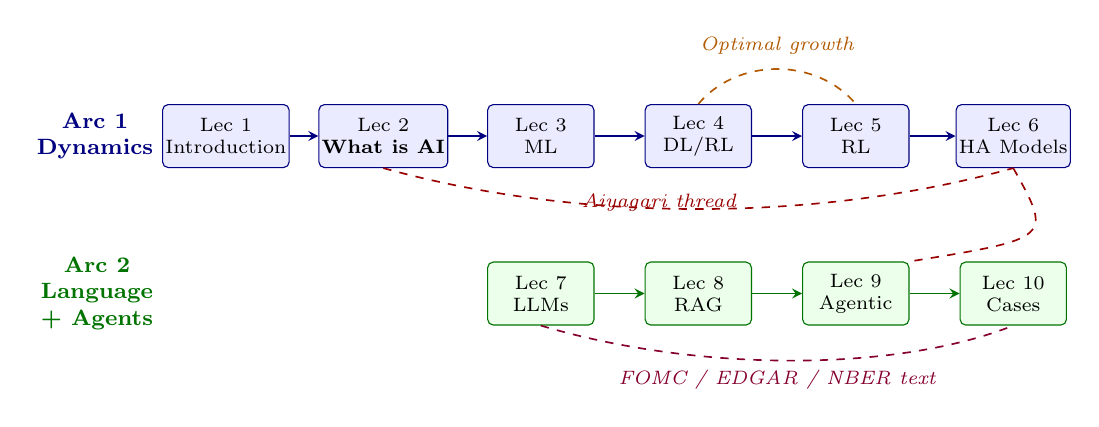
\begin{tikzpicture}[
    every node/.style={font=\scriptsize},
    arc1box/.style={draw=blue!50!black, fill=blue!8, rounded corners=2pt, minimum width=1.35cm, minimum height=0.8cm, align=center, inner sep=1pt},
    arc2box/.style={draw=green!45!black, fill=green!8, rounded corners=2pt, minimum width=1.35cm, minimum height=0.8cm, align=center, inner sep=1pt},
    flowarrow/.style={->, >=stealth, semithick},
    threadlabel/.style={font=\scriptsize\itshape},
]
% Arc 1 row (top)
\node[arc1box] (L1) at (0.0, 1.7) {Lec 1\\Introduction};
\node[arc1box] (L2) at (2.0, 1.7) {Lec 2\\\textbf{What is AI}};
\node[arc1box] (L3) at (4.0, 1.7) {Lec 3\\ML};
\node[arc1box] (L4) at (6.0, 1.7) {Lec 4\\DL/RL};
\node[arc1box] (L5) at (8.0, 1.7) {Lec 5\\RL};
\node[arc1box] (L6) at (10.0, 1.7) {Lec 6\\HA Models};
\draw[flowarrow, blue!50!black] (L1) -- (L2);
\draw[flowarrow, blue!50!black] (L2) -- (L3);
\draw[flowarrow, blue!50!black] (L3) -- (L4);
\draw[flowarrow, blue!50!black] (L4) -- (L5);
\draw[flowarrow, blue!50!black] (L5) -- (L6);

% Arc 2 row (bottom)
\node[arc2box] (L7) at (4.0, -0.3) {Lec 7\\LLMs};
\node[arc2box] (L8) at (6.0, -0.3) {Lec 8\\RAG};
\node[arc2box] (L9) at (8.0, -0.3) {Lec 9\\Agentic};
\node[arc2box] (L10) at (10.0, -0.3) {Lec 10\\Cases};
\draw[flowarrow, green!45!black] (L7) -- (L8);
\draw[flowarrow, green!45!black] (L8) -- (L9);
\draw[flowarrow, green!45!black] (L9) -- (L10);

% Arc labels
\node[anchor=east, align=center, blue!50!black, font=\footnotesize\bfseries] at (-0.8, 1.7) {Arc 1\\Dynamics};
\node[anchor=east, align=center, green!45!black, font=\footnotesize\bfseries] at (-0.8, -0.3) {Arc 2\\Language\\+ Agents};

% Aiyagari thread: Lec 2 -> Lec 6 -> Lec 9
\draw[dashed, red!60!black, semithick] (L2.south) .. controls (4.5, 0.6) and (7.5, 0.6) .. (L6.south);
\draw[dashed, red!60!black, semithick] (L6.south) .. controls (10.5, 0.4) and (10.5, 0.4) .. (L9.north east);
\node[threadlabel, red!60!black] at (5.5, 0.85) {Aiyagari thread};

% Optimal growth thread: Lec 4 -> Lec 5
\draw[dashed, orange!70!black, semithick] (L4.north) .. controls (6.5, 2.7) and (7.5, 2.7) .. (L5.north);
\node[threadlabel, orange!70!black] at (7.0, 2.85) {Optimal growth};

% FOMC/EDGAR thread: Lec 7 -> Lec 8 -> Lec 10
\draw[dashed, purple!70!black, semithick] (L7.south) .. controls (6.0, -1.3) and (8.5, -1.3) .. (L10.south);
\node[threadlabel, purple!70!black] at (7.0, -1.4) {FOMC / EDGAR / NBER text};
\end{tikzpicture}
\end{center}
\vspace{-2mm}
\begin{center}
\footnotesize\textit{Every running example traces multiple lectures. Build the foundation, then re-meet it in agentic form.}
\end{center}
\end{frame}

\begin{frame}{What You Need to Know vs.\ What AI Can Help With}
\begin{itemize}
\item \textbf{What economists must bring:}
\begin{itemize}
    \item Economic intuition: what is the right model, state space, welfare criterion?
    \item Identification: why does this variation estimate a causal effect?
    \item Domain knowledge: what makes FOMC minutes different from random text?
    \item Judgment: when is the AI output trustworthy?
\end{itemize}

\medskip
\item \textbf{What AI can do for you:}
\begin{itemize}
    \item Solve high-dimensional optimization problems (Bellman, ML training)
    \item Process and extract information from large text/data collections
    \item Write, run, and debug code at scale
    \item Synthesize literature and summarize research
\end{itemize}

\medskip
\item \textbf{The Regime Change:}
\begin{itemize}
    \item The bottleneck in research is shifting from \emph{execution} (writing code, computing) to \emph{design} (what question to ask, how to identify it)
    \item Your advantage as an economist: you know what question matters
\end{itemize}
\end{itemize}
\end{frame}

%=============================================================================
\section{Research-Architect Stance \& Tooling}

\sectiondivider{Research-Architect Stance \& Tooling}{You bring the question, the identification, and the judgment; AI supplies throughput}

\begin{frame}{You Are the Research Architect: The 5-Pillar Workflow}
\begin{itemize}
\item Across the ten lectures you build four competencies --- theoretical mastery, technical fluency, AI-augmented implementation, and critical validation. The capstone is where they meet a real problem.
\item \textbf{The 5-pillar workflow --- your scaffold on every project:}
\begin{enumerate}
    \item \textbf{Economic theory} --- state the problem precisely (objective, constraints, equilibrium or estimand).
    \item \textbf{Algorithm design} --- choose the method (VFI vs.\ Euler iteration; WLS; embedding + retrieval; a typed graph).
    \item \textbf{Numerical / empirical technique} --- discretization, weighting, sampling, chunking.
    \item \textbf{Advanced method \& trade-offs} --- accuracy vs.\ speed, bias vs.\ variance, precision vs.\ recall.
    \item \textbf{Code literacy \& validation} --- read every line; benchmark; sanity-check against economics.
\end{enumerate}
\end{itemize}
\begin{takeawaybox}
\footnotesize
\textbf{The stance:} AI handles the bricks --- syntax, boilerplate, data wrangling, refactoring --- while \emph{you} own the theory, the validation, and the interpretation. We are not impressed by code an agent wrote; we are impressed by a correct result you can defend.
\end{takeawaybox}
\end{frame}

\begin{frame}{Replicate First, Explore Second}
\begin{itemize}
\item \textbf{Baseline (the core deliverable):} faithfully \emph{reproduce and verify} a known result --- a classical solution, a published number, or the instructor's reported finding --- on public data or at small scale.
\item \textbf{Stretch (upside):} finding ``something more interesting'' only counts \emph{once the replication validates}. This mirrors how real research works, and how Lec.\ 9--10 teach you to use AI: build the trusted benchmark, \emph{then} extend.
\end{itemize}
\begin{cautionbox}
\footnotesize
\textbf{Validation discipline (non-negotiable).} For every headline result:
(i) re-derive at least one number by hand or in a second tool;
(ii) benchmark against a \emph{known} quantity (a classical solution, a published figure, a standard package);
(iii) run economic sanity checks ($\beta \in (0,1)$; Euler-equation errors below threshold; signs match theory);
(iv) \textbf{never} submit code you have not read end to end.
\end{cautionbox}
\end{frame}

\begin{frame}{Reproducibility Discipline}
\begin{itemize}
\item \textbf{One command should reproduce your results.} The reproducibility package is a graded artifact, not an afterthought.
\end{itemize}
\begin{conceptbox}
\footnotesize
\textbf{Every project ships:}
\begin{itemize}
    \item Git history + \textbf{fixed random seeds}
    \item A pinned environment (\texttt{environment.yml} / \texttt{requirements.txt})
    \item \texttt{CLAUDE.md} --- describes the project for the next agent (and human)
    \item \texttt{AI\_LOG.md} --- a running log of how you used AI: the prompts that mattered, the decisions you made, where the AI was wrong and how you caught it, an honest human-vs-AI split
    \item A \texttt{README} with run instructions, a data dictionary, and recorded access dates
\end{itemize}
\end{conceptbox}
\smallskip
{\footnotesize\textit{The \texttt{AI\_LOG.md} is the evidence that you were the architect, not the consumer.}}
\end{frame}

\begin{frame}{Tools You'll Use}
\begin{itemize}
\item \textbf{Minimum:} VS Code + Python. Everything in this course runs there --- no Google/Colab required.
\item \textbf{Encouraged (the point of the course):} use AI as a \emph{partner, not a ghostwriter} --- Claude Code, an IDE agent, or a chat model across the whole pipeline: scoping, data acquisition, coding, debugging, drafting. What is \emph{not} allowed is shipping anything you cannot read, explain, and defend.
\end{itemize}
\begin{conceptbox}
\footnotesize
\textbf{For students in China.} The labs run top-to-bottom \textbf{offline}; setup uses \textbf{Tsinghua (TUNA) mirrors} for conda/pip. Start with \texttt{Labs/Lec01\_02\_Lab\_Getting\_Started.ipynb}: install Python + PyTorch in VS Code and plot Stanford \emph{AI Index} data (AI vs.\ human experts, inference cost, adoption speed) --- the very figures from T1.1, now in your own hands.
\end{conceptbox}
\end{frame}

%=============================================================================
\section{Capstone Projects}

\sectiondivider{Capstone Projects}{Four tracks, replication-first grading --- the stretch is upside}

\begin{frame}{Capstone: Four Tracks (Pick One)}
\compacttables
\begin{center}\footnotesize
\begin{tabular}{clcc}
\toprule
\textbf{Track} & \textbf{One-line pitch} & \textbf{Builds on} & \textbf{Instructor research} \\
\midrule
\textbf{A} & Optimal growth via deep learning & Lec.\ 1,3,4,5 & (thematic) \\
\textbf{B} & Build \& validate an AI-exposure index & Lec.\ 2,7,10 & AI-index (WIP) \\
\textbf{C} & Text as economic data (+ small RAG) & Lec.\ 7,8 & (adjacent) \\
\textbf{D} & AI-for-research infrastructure & Lec.\ 8,9,10 & GRAM / GraphRAG (WIP) \\
\bottomrule
\end{tabular}
\end{center}
\smallskip
\begin{itemize}\footnotesize
\item \textbf{B} reconstructs, on public data, the task-level Anthropic Economic Index $\times$ O\*NET exposure index previewed in \textbf{T1.2} (the live measurement example).
\item \textbf{D} engages the \textbf{GRAM} typed-retrieval project previewed in \textbf{T1.2} (Case B).
\item Tracks B, C, D touch \emph{active, unpublished} research --- findings are labeled preliminary / WIP.
\end{itemize}
\end{frame}

\begin{frame}{Capstone Tracks: Baseline \& Stretch}
\footnotesize
\begin{description}
\item[A --- Optimal Growth via DL] \emph{Baseline:} solve the optimal growth model with a neural net (Euler-residual loss and/or actor--critic) and match the classical VFI / time-iteration benchmark on Euler errors. \emph{Stretch:} add a stochastic TFP shock or a second state; or an ``AI-as-capital'' productivity twist.
\smallskip
\item[B --- AI-Exposure Index \textmd{(WIP)}] \emph{Baseline:} rebuild the occupation-level index from the Anthropic Economic Index $\times$ O\*NET ($G$, $|G|$, importance-weighted intensity) and verify the structure from T1.2. \emph{Stretch:} link to IPUMS-CPS / BLS OES employment (WLS, robust SEs); probe the usage\,$\times$\,concentration interaction.
\smallskip
\item[C --- Text as Economic Data] \emph{Baseline:} turn a corpus (FOMC / 10-K / news) into a validated measure --- a lexical \emph{and} an embedding version --- plus a small RAG (chunk\,$\to$\,embed\,$\to$\,store\,$\to$\,retrieve), validated against an external benchmark out of sample. \emph{Stretch:} a novel index or a head-to-head where embeddings beat the baseline.
\smallskip
\item[D --- AI-for-Research Infra \textmd{(WIP)}] \emph{Baseline:} either a mini condition-aware GraphRAG (flat RAG vs.\ typed-retrieval ablation) or a validated Claude Code skill (explicit phases, confidence gates, quote verification). \emph{Stretch:} the supervised, confidential GRAM comparison; or a human-vs-skill evaluation.
\end{description}
\end{frame}

\begin{frame}{Logistics \& Grading}
\begin{columns}[T]
\column{0.46\textwidth}
\footnotesize
\textbf{Teams of 2--4} (mix theory + data/code).\\[0.4em]
\textbf{Milestones:}
\begin{itemize}
    \item \textbf{M1} Proposal --- track, question, the \emph{specific} result to replicate, data, division of labor
    \item \textbf{M2} Data / infra up --- pipeline runs; benchmark in hand; repo scaffolded
    \item \textbf{M3} Replication verified --- the core grade; stretch scoped
    \item \textbf{M4} Paper, repo, talk, peer-review report
\end{itemize}
\column{0.52\textwidth}
\compacttables
\scriptsize
\begin{tabular}{lc}
\toprule
\textbf{Dimension} & \textbf{Pts} \\
\midrule
Economic framing \& question & 15 \\
Replication correctness & 20 \\
Validation rigor & 20 \\
Reproducibility \& provenance & 15 \\
AI-collaboration quality & 10 \\
Communication & 10 \\
Peer-review quality & 10 \\
\midrule
Stretch finding (bonus) & +10 \\
\bottomrule
\end{tabular}
\end{columns}
\smallskip
{\footnotesize\textit{A project that only replicates --- correctly, with rigorous validation and clean reproduction --- earns a strong grade. The stretch is upside.}}
\end{frame}

%=============================================================================
\begin{frame}{The Companion Textbook: Full Topic Map}
\noindent{\footnotesize\textit{Miao \& Feng, \emph{Artificial Intelligence for Economists} (Higher Education Press, 2027) --- 16 chapters in six parts. This course samples the book; here is its full coverage.}}\par
\smallskip
\begin{columns}[T]
\column{0.5\textwidth}
\footnotesize
\textbf{\textcolor{RedTitle}{Part I --- Introduction \& Background}}\\
\textbf{1.}~AI as research infrastructure \textperiodcentered\ \textbf{2.}~a short history of AI \& the new data environment
\smallskip

\textbf{\textcolor{RedTitle}{Part II --- Foundations}}\\
\textbf{3.}~the logic of machine learning \textperiodcentered\ \textbf{4.}~mathematical foundations of ML \textperiodcentered\ \textbf{5.}~research engineering
\smallskip

\textbf{\textcolor{RedTitle}{Part III --- Machine-Learning Methods}}\\
\textbf{6.}~supervised learning (prediction) \textperiodcentered\ \textbf{7.}~unsupervised learning (structure) \textperiodcentered\ \textbf{8.}~double ML: prediction\,$\to$\,causality \textperiodcentered\ \textbf{9.}~ML-enhanced causal identification

\column{0.5\textwidth}
\footnotesize
\textbf{\textcolor{RedTitle}{Part IV --- Deep Learning}}\\
\textbf{10.}~neural-network foundations \textperiodcentered\ \textbf{11.}~economic applications of deep learning
\smallskip

\textbf{\textcolor{RedTitle}{Part V --- Reinforcement Learning}}\\
\textbf{12.}~foundations of reinforcement learning \textperiodcentered\ \textbf{13.}~core RL algorithms
\smallskip

\textbf{\textcolor{RedTitle}{Part VI --- Text, Language Models \& AI-Assisted Research}}\\
\textbf{14.}~text representation \& language-model basics \textperiodcentered\ \textbf{15.}~large language model applications \textperiodcentered\ \textbf{16.}~retrieval-augmented generation \& agents
\end{columns}
\smallskip
\begin{takeawaybox}\footnotesize
\textbf{Course vs.\ book.} These ten lectures follow the \emph{dynamics} and \emph{language} arcs --- roughly Parts IV--VI. The book widens the lens with Part II's \emph{foundations} and Part III's full \emph{ML-methods} toolkit --- supervised/unsupervised learning and \textbf{double ML / causal forests} --- the prediction-and-causal-inference methods every empirical economist now needs.
\end{takeawaybox}
\end{frame}

\begin{frame}{Lecture 1, Complete: One Map, Three Acts}
\textbf{The claim is framed, proven, and handed to you: AI is cognitive capital, it already does research, and this course is where you make it yours.}

\LecOneMap{0}

\vspace{0.05cm}
\footnotesize\textit{Bring the question, the identification, and the judgment; let AI supply throughput --- the stance every later lecture assumes.}
\end{frame}

\begin{frame}{Preview: What Lec.\ 2 Delivers}
\begin{itemize}
\item \textbf{Lecture 1 set the why and the how:} AI as fast, cheap, widely adopted cognitive capital (T1.1); AI already \emph{doing} frontier research (T1.2); and how this course works --- the architect stance, tooling, and capstone (T1.3).
\item \textbf{Lecture 2 --- ``What is AI?''} opens the technique families you will use: machine learning, deep learning, reinforcement learning, LLMs, and agentic AI --- and, crucially, \emph{where AI fails} (predictive and generative), so you wield it as powerful but bounded.
\end{itemize}
\begin{takeawaybox}
\footnotesize
You are the Research Architect: bring the question, the identification, and the judgment; let AI supply throughput. Next we open the toolbox.
\end{takeawaybox}
\end{frame}

\begin{frame}{Summary}
\begin{enumerate}
\item \textbf{Why now:} AI is cheap, fast, and diffusing at record speed --- a \emph{candidate} general-purpose technology moving on a timescale of months (snapshot: early 2026).

\medskip
\item \textbf{Cognitive capital:} AI is \emph{non-rival cognitive capital} --- entering growth through automation ($K$), idea production ($A$), and a new intangible stock.

\medskip
\item \textbf{The measurement gap:} task-level gains do not auto-sum to macro TFP --- bottleneck tasks and mismeasured intangibles keep aggregate estimates modest (Acemoglu 2024).

\medskip
\item \textbf{AI already does research:} DeepRamsey co-developed a dynamic model; GRAM showed \emph{context, not capability}, is the bottleneck --- with causation as the standing guardrail.

\medskip
\item \textbf{You are the Research Architect:} bring the question, the identification, and the judgment; let AI supply throughput --- the stance the replication-first capstone trains.

\medskip
\item \textbf{Next:} Lec.\ 2 opens the toolbox --- the predictive stack (T1) and the generative \& agentic stack (T2), each with where it fails.
\end{enumerate}
\end{frame}

\end{document}
